% Options for packages loaded elsewhere
\PassOptionsToPackage{unicode}{hyperref}
\PassOptionsToPackage{hyphens}{url}
\PassOptionsToPackage{dvipsnames,svgnames,x11names}{xcolor}
%
\documentclass[
]{book}
\usepackage{amsmath,amssymb}
\usepackage{lmodern}
\usepackage{iftex}
\ifPDFTeX
  \usepackage[T1]{fontenc}
  \usepackage[utf8]{inputenc}
  \usepackage{textcomp} % provide euro and other symbols
\else % if luatex or xetex
  \usepackage{unicode-math}
  \defaultfontfeatures{Scale=MatchLowercase}
  \defaultfontfeatures[\rmfamily]{Ligatures=TeX,Scale=1}
\fi
% Use upquote if available, for straight quotes in verbatim environments
\IfFileExists{upquote.sty}{\usepackage{upquote}}{}
\IfFileExists{microtype.sty}{% use microtype if available
  \usepackage[]{microtype}
  \UseMicrotypeSet[protrusion]{basicmath} % disable protrusion for tt fonts
}{}
\makeatletter
\@ifundefined{KOMAClassName}{% if non-KOMA class
  \IfFileExists{parskip.sty}{%
    \usepackage{parskip}
  }{% else
    \setlength{\parindent}{0pt}
    \setlength{\parskip}{6pt plus 2pt minus 1pt}}
}{% if KOMA class
  \KOMAoptions{parskip=half}}
\makeatother
\usepackage{xcolor}
\usepackage{color}
\usepackage{fancyvrb}
\newcommand{\VerbBar}{|}
\newcommand{\VERB}{\Verb[commandchars=\\\{\}]}
\DefineVerbatimEnvironment{Highlighting}{Verbatim}{commandchars=\\\{\}}
% Add ',fontsize=\small' for more characters per line
\usepackage{framed}
\definecolor{shadecolor}{RGB}{248,248,248}
\newenvironment{Shaded}{\begin{snugshade}}{\end{snugshade}}
\newcommand{\AlertTok}[1]{\textcolor[rgb]{0.94,0.16,0.16}{#1}}
\newcommand{\AnnotationTok}[1]{\textcolor[rgb]{0.56,0.35,0.01}{\textbf{\textit{#1}}}}
\newcommand{\AttributeTok}[1]{\textcolor[rgb]{0.77,0.63,0.00}{#1}}
\newcommand{\BaseNTok}[1]{\textcolor[rgb]{0.00,0.00,0.81}{#1}}
\newcommand{\BuiltInTok}[1]{#1}
\newcommand{\CharTok}[1]{\textcolor[rgb]{0.31,0.60,0.02}{#1}}
\newcommand{\CommentTok}[1]{\textcolor[rgb]{0.56,0.35,0.01}{\textit{#1}}}
\newcommand{\CommentVarTok}[1]{\textcolor[rgb]{0.56,0.35,0.01}{\textbf{\textit{#1}}}}
\newcommand{\ConstantTok}[1]{\textcolor[rgb]{0.00,0.00,0.00}{#1}}
\newcommand{\ControlFlowTok}[1]{\textcolor[rgb]{0.13,0.29,0.53}{\textbf{#1}}}
\newcommand{\DataTypeTok}[1]{\textcolor[rgb]{0.13,0.29,0.53}{#1}}
\newcommand{\DecValTok}[1]{\textcolor[rgb]{0.00,0.00,0.81}{#1}}
\newcommand{\DocumentationTok}[1]{\textcolor[rgb]{0.56,0.35,0.01}{\textbf{\textit{#1}}}}
\newcommand{\ErrorTok}[1]{\textcolor[rgb]{0.64,0.00,0.00}{\textbf{#1}}}
\newcommand{\ExtensionTok}[1]{#1}
\newcommand{\FloatTok}[1]{\textcolor[rgb]{0.00,0.00,0.81}{#1}}
\newcommand{\FunctionTok}[1]{\textcolor[rgb]{0.00,0.00,0.00}{#1}}
\newcommand{\ImportTok}[1]{#1}
\newcommand{\InformationTok}[1]{\textcolor[rgb]{0.56,0.35,0.01}{\textbf{\textit{#1}}}}
\newcommand{\KeywordTok}[1]{\textcolor[rgb]{0.13,0.29,0.53}{\textbf{#1}}}
\newcommand{\NormalTok}[1]{#1}
\newcommand{\OperatorTok}[1]{\textcolor[rgb]{0.81,0.36,0.00}{\textbf{#1}}}
\newcommand{\OtherTok}[1]{\textcolor[rgb]{0.56,0.35,0.01}{#1}}
\newcommand{\PreprocessorTok}[1]{\textcolor[rgb]{0.56,0.35,0.01}{\textit{#1}}}
\newcommand{\RegionMarkerTok}[1]{#1}
\newcommand{\SpecialCharTok}[1]{\textcolor[rgb]{0.00,0.00,0.00}{#1}}
\newcommand{\SpecialStringTok}[1]{\textcolor[rgb]{0.31,0.60,0.02}{#1}}
\newcommand{\StringTok}[1]{\textcolor[rgb]{0.31,0.60,0.02}{#1}}
\newcommand{\VariableTok}[1]{\textcolor[rgb]{0.00,0.00,0.00}{#1}}
\newcommand{\VerbatimStringTok}[1]{\textcolor[rgb]{0.31,0.60,0.02}{#1}}
\newcommand{\WarningTok}[1]{\textcolor[rgb]{0.56,0.35,0.01}{\textbf{\textit{#1}}}}
\usepackage{longtable,booktabs,array}
\usepackage{calc} % for calculating minipage widths
% Correct order of tables after \paragraph or \subparagraph
\usepackage{etoolbox}
\makeatletter
\patchcmd\longtable{\par}{\if@noskipsec\mbox{}\fi\par}{}{}
\makeatother
% Allow footnotes in longtable head/foot
\IfFileExists{footnotehyper.sty}{\usepackage{footnotehyper}}{\usepackage{footnote}}
\makesavenoteenv{longtable}
\usepackage{graphicx}
\makeatletter
\def\maxwidth{\ifdim\Gin@nat@width>\linewidth\linewidth\else\Gin@nat@width\fi}
\def\maxheight{\ifdim\Gin@nat@height>\textheight\textheight\else\Gin@nat@height\fi}
\makeatother
% Scale images if necessary, so that they will not overflow the page
% margins by default, and it is still possible to overwrite the defaults
% using explicit options in \includegraphics[width, height, ...]{}
\setkeys{Gin}{width=\maxwidth,height=\maxheight,keepaspectratio}
% Set default figure placement to htbp
\makeatletter
\def\fps@figure{htbp}
\makeatother
\setlength{\emergencystretch}{3em} % prevent overfull lines
\providecommand{\tightlist}{%
  \setlength{\itemsep}{0pt}\setlength{\parskip}{0pt}}
\setcounter{secnumdepth}{5}
\usepackage{booktabs}
\ifLuaTeX
  \usepackage{selnolig}  % disable illegal ligatures
\fi
\usepackage[]{natbib}
\bibliographystyle{plainnat}
\IfFileExists{bookmark.sty}{\usepackage{bookmark}}{\usepackage{hyperref}}
\IfFileExists{xurl.sty}{\usepackage{xurl}}{} % add URL line breaks if available
\urlstyle{same} % disable monospaced font for URLs
\hypersetup{
  pdftitle={R Bootcamp - How to use R for Data Science},
  pdfauthor={Yigit Aydede},
  colorlinks=true,
  linkcolor={Maroon},
  filecolor={Maroon},
  citecolor={Blue},
  urlcolor={cyan},
  pdfcreator={LaTeX via pandoc}}

\title{R Bootcamp - How to use R for Data Science}
\author{\href{https://yaydede.github.io/}{Yigit Aydede}}
\date{2022-10-12}

\usepackage{amsthm}
\newtheorem{theorem}{Theorem}[chapter]
\newtheorem{lemma}{Lemma}[chapter]
\newtheorem{corollary}{Corollary}[chapter]
\newtheorem{proposition}{Proposition}[chapter]
\newtheorem{conjecture}{Conjecture}[chapter]
\theoremstyle{definition}
\newtheorem{definition}{Definition}[chapter]
\theoremstyle{definition}
\newtheorem{example}{Example}[chapter]
\theoremstyle{definition}
\newtheorem{exercise}{Exercise}[chapter]
\theoremstyle{definition}
\newtheorem{hypothesis}{Hypothesis}[chapter]
\theoremstyle{remark}
\newtheorem*{remark}{Remark}
\newtheorem*{solution}{Solution}
\begin{document}
\maketitle

{
\hypersetup{linkcolor=}
\setcounter{tocdepth}{1}
\tableofcontents
}
\hypertarget{about}{%
\chapter*{About}\label{about}}
\addcontentsline{toc}{chapter}{About}

This book covers basics to learn R for Data Science. It is designed for MBAN students.

We also have a companion R package named \texttt{RBootcamp}, containing the data sets used as well as interactive exercises for each part.


\includegraphics[width=4.16667in,height=5.72917in]{png/cover.png}

\hypertarget{why-r}{%
\section*{Why R?}\label{why-r}}
\addcontentsline{toc}{section}{Why R?}

R is both a programming language and software environment for statistical computing, which is free and open-source.

With ever increasing availability of large amounts of data, it is critical to have the ability to analyze the data and learn from it for making informed decisions. Familiarity with software such as R allows users to visualize data, run statistical tests, and apply machine learning algorithms. Even if you already know other software, there are still good reasons to learn R:

\begin{enumerate}
\def\labelenumi{\arabic{enumi}.}
\item
  \textbf{R is free.} If your future employer does not already have R installed, you can always download it for free, unlike other proprietary software packages that require expensive licenses. You can always have access to R on your computer.
\item
  \textbf{R gives you access to cutting-edge technology.} Top researchers develop statistical learning methods in R, and new algorithms are constantly added to the list of packages you can download.
\item
  \textbf{R is a useful skill.} Employers that value analytics recognize R as useful and important. If for no other reason, learning R is worthwhile to help \textbf{boost your resume.}
\end{enumerate}

Here is a very good article about R and Programming that everybody should read: \href{http://gilesd-j.com/2019/01/07/7-reasons-for-policy-professionals-to-get-pumped-about-r-programming-in-2019/}{7 Reasons for policy professionals to get into R programming in 2019} \citep{Jones_2019}.

\hypertarget{license}{%
\section*{License}\label{license}}
\addcontentsline{toc}{section}{License}

\begin{figure}
\centering

\includegraphics{png/cc.png}
\caption{This work is licensed under a \href{http://creativecommons.org/licenses/by-nc-sa/4.0/}{Creative Commons Attribution-NonCommercial-ShareAlike 4.0 International License}.}
\end{figure}

\hypertarget{introduction}{%
\chapter{Introduction}\label{introduction}}

The following sections will serve as an introduction to the R basics that could be used in data analytics. At the beginning, these introductory R subjects may feel like an overwhelming amount of information. The leaning curve will be steeper as practice more. You should try all of the codes from these examples and solve the practice exercises.

R is used both for software development and data analysis. We will not use it for software development but apply some concepts in that area. Our main goal will be to analyze data, but we will also perform programming exercises that help illustrate certain algorithmic concepts.

What we will review in this Chapter:

\begin{enumerate}
\def\labelenumi{\arabic{enumi}.}
\tightlist
\item
  \textbf{R, RStudio, and R Packages},
\item
  \textbf{Starting with RStudio},
\item
  \textbf{Working Directory},
\item
  \textbf{Data Types and Structures (Vectors and Matrices)},
\item
  \textbf{R-Style Guide}
\end{enumerate}

\hypertarget{installation-of-r-rstudio-and-r-packages}{%
\section{Installation of R, RStudio and R Packages}\label{installation-of-r-rstudio-and-r-packages}}

To get started, you will need to install two pieces of software:

\textbf{R}, the actual programming language: \href{https://cran.r-project.org}{\textbf{Download it from here.}}
-- Chose your operating system, and select the most recent version.

\textbf{RStudio}, an excellent integrated development environment (IDE) for working with R, an interface used to interact with R: \href{https://www.rstudio.com}{\textbf{Download it from here.}} Throughout this book, you will use RStudio instead of R to learn R programming.

\hypertarget{rstudio}{%
\section{RStudio}\label{rstudio}}

\includegraphics[width=15.15in]{png/Rstudio}

Source Pane, click on the plus sign in the top left corner. From the drop-down menu, select \textbf{R Script} . As shown in that dropdown menu, you can also open an R Script by pressing \textbf{Ctrl+Shift+N}. You should now see the screen above.

The \textbf{Console Pane} is the interface to R. If you opened R directly instead of opening RStudio, you would see just this console. You can type commands directly in the console. The console displays the results of any command you run. For example, type 2+4 in the command line and press enter. You should see the command you typed, the result of the command, and a new command line.

\includegraphics[width=8.24in]{png/Rstudio2}

To clear the console, you press \textbf{Ctrl+L} or type \textbf{cat(``\textbackslash014'')} in the command line.

R code can be entered into the command line directly (in Console Pane) or saved to a script (Source Pane).

Let's try some coding.

\begin{Shaded}
\begin{Highlighting}[]
\DecValTok{2} \SpecialCharTok{+} \DecValTok{3} \CommentTok{\#write this on the command line and hit Enter}
\end{Highlighting}
\end{Shaded}

\begin{verbatim}
## [1] 5
\end{verbatim}

Now write the same line into the script in Source Pane and \textbf{run} it

\includegraphics[width=4.75in]{png/Rstudio5}

The \textbf{Source Pane} is a text editor where you can type your code before running it. You can save your code in a text file called a script. Scripts have typically file names with the extension \textbf{.R}. Any text shown in green is a comment in the script. You write a comment by adding a \textbf{\#} to an RScript. Anything to the right of a \texttt{\#} is considered a comment and is thus ignored by R when running code. Place your cursor anywhere on the first few lines of code and click \textbf{Run}. You can also run code by pressing \textbf{Ctrl+Enter}.

\includegraphics[width=8.12in]{png/Rstudio3}

The \textbf{Environment Pane} includes an Environment, a History tab, and a Connections tab. The Connections tab makes it easy to connect to any data source on your system.

The Environment tab displays any objects that you have created during your R session. For example, if we create three variables: \(x\), \(y\), and \(z\), R stored those variables as objects so that you can see them in the Environment pane.

To do object assignments, you need to assign value(s) to a name via the assignment operator, which will create a new object with a name.

\begin{Shaded}
\begin{Highlighting}[]
\NormalTok{x }\OtherTok{\textless{}{-}} \DecValTok{5}
\NormalTok{y }\OtherTok{\textless{}{-}}\NormalTok{ x}\SpecialCharTok{*}\FloatTok{1.5}
\NormalTok{z }\OtherTok{\textless{}{-}}\NormalTok{ x }\SpecialCharTok{{-}}\NormalTok{ y}\SpecialCharTok{*}\DecValTok{3}
\FunctionTok{ls}\NormalTok{()}
\end{Highlighting}
\end{Shaded}

\begin{verbatim}
## [1] "x" "y" "z"
\end{verbatim}

We will discuss R objects in more detail later. If you want to see a list of all objects in the current session, type \texttt{ls()} in the command line. You can remove an individual object from the environment with the \texttt{rm()} command. For example, remove \(x\) by typing \texttt{rm(x)} in the command line. You can remove all objects from the environment by clicking or typing \texttt{rm(list=ls())} in the command line. The History tab keeps a record of all the commands you have run. To copy a command from the history into the console, select the command and press Enter.

The \textbf{Files Pane} includes several tabs that provide useful information. The Files tab displays the contents of your working directory. The Plot tab shows all graphs that you have created. The Packages tab displays the R packages that you have installed in your System Library.

\hypertarget{packages}{%
\section{Packages}\label{packages}}

An R package typically includes code, data, documentation for the package and functions inside, and tests to check everything works as it should. Check to see if the package \texttt{moments} has been installed. If you cannot find it, you need to install it by using the command \texttt{install.packages("moments")}. Once you have installed the package, you need to load it using the command \texttt{library(moments)}. Or you can use install tab and follow the instructions and the go to package to check it to activate as shown below.

\includegraphics[width=8.12in]{png/Rstudio4}

The help tab has built-in documentation for packages and functions in R. The help is automatically available for any loaded packages. You can access that file by typing \texttt{help(mean)} or \texttt{?mean} in the command line. You can also use the search bar in the help tab.

The packages can be installed from sources other than CRAN. For example, in this book we will use \texttt{RBootcamp} which is not located on CRAN

\begin{Shaded}
\begin{Highlighting}[]
\CommentTok{\#install.packages("remotes")}
\CommentTok{\#remotes::install\_github("yaydede/RBootcamp")}
\end{Highlighting}
\end{Shaded}

One of the most difficult things to do when learning R is to know how to find help. Your very first helper should be \textbf{Google} where you post your error message or a short description of your issue. The ability to solve problems using this method is quickly becoming an extremely valuable skill.

\textbf{Do not be discouraged by running into errors and difficulties when learning R. It is simply part of the learning process.}

The Viewer tab displays HTML output. R packages such as R Markdown and Shiny create HTML outputs that you can view in the Viewer tab. We'll see it later.

\hypertarget{working-directory}{%
\section{Working directory}\label{working-directory}}

Without further specification, files will be loaded from and saved to the working directory. The functions \texttt{getwd()} and \texttt{setwd()} will get and set the working directory, respectively.

\begin{Shaded}
\begin{Highlighting}[]
\FunctionTok{getwd}\NormalTok{()}
\end{Highlighting}
\end{Shaded}

\begin{verbatim}
## [1] "/Users/yigitaydede/Dropbox/Documents/Courses/MBAN/RBootcamps/Bootcamp_book"
\end{verbatim}

\begin{Shaded}
\begin{Highlighting}[]
\CommentTok{\#setwd("Book2022")}

\CommentTok{\#List all the objects in your local workspace using}
\FunctionTok{ls}\NormalTok{()}
\end{Highlighting}
\end{Shaded}

\begin{verbatim}
## [1] "x" "y" "z"
\end{verbatim}

\begin{Shaded}
\begin{Highlighting}[]
\CommentTok{\#List all the files in your working directory using list.files() or }
\FunctionTok{dir}\NormalTok{()}
\end{Highlighting}
\end{Shaded}

\begin{verbatim}
##  [1] "_book"                  "_bookdown_files"        "_bookdown.yml"         
##  [4] "_main_files"            "_output.yml"            "01-intro.Rmd"          
##  [7] "02-cross-refs_files"    "02-cross-refs.Rmd"      "03-parts.Rmd"          
## [10] "04-citations.Rmd"       "05-blocks.Rmd"          "06-share.Rmd"          
## [13] "07-references.Rmd"      "Book_for_RBootcamp.log" "Book_for_RBootcamp.rds"
## [16] "book.bib"               "Bootcamp_book.Rproj"    "docs"                  
## [19] "index.md"               "index.Rmd"              "packages.bib"          
## [22] "png"                    "preamble.tex"           "README.md"             
## [25] "render16a06589614b.rds" "style.css"
\end{verbatim}

\begin{Shaded}
\begin{Highlighting}[]
\CommentTok{\#As we go through this lesson, you should be examining the help page }
\CommentTok{\#for each new function. Check out the help page for list.files with the}
\CommentTok{\#command}
\NormalTok{?list.files}
\CommentTok{\#or}
\FunctionTok{help}\NormalTok{(}\StringTok{"list.files"}\NormalTok{)}

\CommentTok{\#Using the args() function on a function name is also a handy way to }
\CommentTok{\#see what arguments a function can take.}
\FunctionTok{args}\NormalTok{(list.files)}
\end{Highlighting}
\end{Shaded}

\begin{verbatim}
## function (path = ".", pattern = NULL, all.files = FALSE, full.names = FALSE, 
##     recursive = FALSE, ignore.case = FALSE, include.dirs = FALSE, 
##     no.. = FALSE) 
## NULL
\end{verbatim}

For this bootcamp, I would suggest to create a RStudio Project in your local driver. RStudio projects make it straightforward to divide your work into multiple contexts, each with their own working directory, workspace, history, and source documents.

RStudio projects are associated with R working directories. You can create an RStudio project:

\begin{itemize}
\tightlist
\item
  In a brand new directory
\item
  In an existing directory where you already have R code and data
\item
  By cloning a version control (Git or Subversion) repository
\end{itemize}

To create a new project in the RStudio, use the Create Project command (available on the Projects menu and on the global toolbar)

\hypertarget{hints}{%
\section{Hints}\label{hints}}

\begin{itemize}
\tightlist
\item
  R distinguishes upper case from lower case letters. Thus a variable named \texttt{X} differs from another variable named \texttt{x}.
\item
  The way to learn programming is through practice. The learning curve to R is not bad. You may struggle a bit in the process, but the skills learned will be invaluable for you in the future.
\item
  There are many ways to write a code to solve the same thing. You can develop your own style. But, if you see nother and better code, try to learn from others!
\item
  There are many option that you can customize R Studio. Check out Tools \textgreater{} Global Options \textgreater{} General tab in the menu bar of RStudio.
\item
  Before you start coding, draft a plan to address the question at hand.
\item
  There is convention in writing codes. Try to adhere these accepted styles.
\item
  Comment your code properly (using a \# sign at the beginning of each line). Good documentation is a great reminder what you have done. Believe me you will forget later the lines in the your own script.
\item
  The character \texttt{\textgreater{}} in the R Console indicates that R is ready for you to enter a command.\\
\item
  Do not overwrite the original data set and variables. Create new data sets just to be sure, especially when taking a subset from that data set.
\end{itemize}

\hypertarget{console-or-script}{%
\section{Console or Script?}\label{console-or-script}}

The Script Window is the place to enter and run your code so that it is easily edited and saved for future use. You create new R Script by clicking on File \textgreater{} New File \textgreater{} R Script in the RStudio menu bar.

To execute your code in the R script, you can either highlight the code and click on Run, or you can highlight the code and press CTRL + Enter on your keyboard.

If you prefer, you can enter code directly in the Console Window and click Enter. The commands that you run will be shown in the History Window on the top right of RStudio. You can save these commands for future use.

Or, to find the older commands in the console, use the upper arrow to get them again \ldots{}

Make sure you save your code. With your code, you can always regenerate your workspace but it could take a little time. Or you can save your workspace which allows you to start where you left off, with all of the variables you created and renamed saved.

Your code (in your script window) is saved by clicking the SAVE button in the RStudio menu bar. The code will be saved in the working directory. See 2.1 for setting and getting the working directory.

\hypertarget{r-as-a-calculator}{%
\section{R as a calculator}\label{r-as-a-calculator}}

At a very basic level, we can use R as a calculator.

See \texttt{Lesson1} in our package \texttt{Rbootcamp}:

\begin{Shaded}
\begin{Highlighting}[]
\FunctionTok{library}\NormalTok{(RBootcamp)}
\CommentTok{\#learnr::run\_tutorial("Lesson1", "RBootcamp")}
\end{Highlighting}
\end{Shaded}

\hypertarget{data-object-types}{%
\section{Data \& Object Types}\label{data-object-types}}

R has a number of basic data types.

\textbf{Numeric}: Also known as Double. The default type when dealing with numbers. 1,1.0,42.5\\
\textbf{Integer}: 1L,2L,42L\\
\textbf{Complex}: 4 + 2i\\
\textbf{Logical}: Two possible values: TRUE and FALSE. NA is also considered logical.\\
\textbf{Character}:``a'',``Statistics'',``1plus2.''

R also has a number of basic data structures. A data structure is either \textbf{homogeneous} (all elements are of the same data type) or \textbf{heterogeneous} (elements can be of more than one data type): You can think each data structure as \textbf{data container} (object types) where you data is stored. Here are the main ``container'' or data structures. Think it as Stata or Excel spread-sheets.

\textbf{Vector}: 1 dimension (column OR row) and homogeneous. That is every element of the vector has to be the same type. Each vector can be thought of as a variable.\\
\textbf{Matrix}: 2 dimensions (column AND row) and homogeneous. That is every element of the matrix has to be the same type.\\
\textbf{Data Frame}: 2 dimensions (column AND row) and heterogeneous. That is every element of the data frame doesn't have to be the same type. This is the main difference between a matrix and a data frame. Data frames are the most common data structure in any data analysis.\\
\textbf{List}: 1 dimension and heterogeneous. Data can be multiple data structures.\\
\textbf{Array}: 3+ dimensions and homogeneous.

\hypertarget{vectors}{%
\chapter{Vectors}\label{vectors}}

Many operations in R make heavy use of vectors. Possibly the most common way to create a vector in R is using the \texttt{c()} function, which is short for ``combine.'' As the name suggests, it combines a list of elements separated by commas.

\begin{Shaded}
\begin{Highlighting}[]
\FunctionTok{c}\NormalTok{(}\DecValTok{1}\NormalTok{, }\DecValTok{5}\NormalTok{, }\DecValTok{0}\NormalTok{, }\SpecialCharTok{{-}}\DecValTok{1}\NormalTok{)}
\end{Highlighting}
\end{Shaded}

\begin{verbatim}
## [1]  1  5  0 -1
\end{verbatim}

If we would like to store this vector in a \textbf{variable} we can do so with the assignment operator \texttt{\textless{}-} or \texttt{=}. But the convention is \texttt{\textless{}-}

\begin{Shaded}
\begin{Highlighting}[]
\NormalTok{x }\OtherTok{\textless{}{-}} \FunctionTok{c}\NormalTok{(}\DecValTok{1}\NormalTok{, }\DecValTok{5}\NormalTok{, }\DecValTok{0}\NormalTok{, }\SpecialCharTok{{-}}\DecValTok{1}\NormalTok{)}
\NormalTok{z }\OtherTok{=} \FunctionTok{c}\NormalTok{(}\DecValTok{1}\NormalTok{, }\DecValTok{5}\NormalTok{, }\DecValTok{0}\NormalTok{, }\SpecialCharTok{{-}}\DecValTok{1}\NormalTok{)}
\NormalTok{x}
\end{Highlighting}
\end{Shaded}

\begin{verbatim}
## [1]  1  5  0 -1
\end{verbatim}

\begin{Shaded}
\begin{Highlighting}[]
\NormalTok{z}
\end{Highlighting}
\end{Shaded}

\begin{verbatim}
## [1]  1  5  0 -1
\end{verbatim}

Note that scalars do not exists in R. They are simply vectors of length 1.

\begin{Shaded}
\begin{Highlighting}[]
\NormalTok{y }\OtherTok{\textless{}{-}} \DecValTok{24}  \CommentTok{\#this a vector with 1 element, 24}
\end{Highlighting}
\end{Shaded}

\hypertarget{one-type-same-type}{%
\section{One type, same type}\label{one-type-same-type}}

Because vectors must contain elements that are all the same type, R will automatically coerce to a single type when attempting to create a vector that combines multiple types.

\begin{Shaded}
\begin{Highlighting}[]
\FunctionTok{c}\NormalTok{(}\DecValTok{10}\NormalTok{, }\StringTok{"Machine Learning"}\NormalTok{, }\ConstantTok{FALSE}\NormalTok{)}
\end{Highlighting}
\end{Shaded}

\begin{verbatim}
## [1] "10"               "Machine Learning" "FALSE"
\end{verbatim}

\begin{Shaded}
\begin{Highlighting}[]
\FunctionTok{c}\NormalTok{(}\DecValTok{10}\NormalTok{, }\ConstantTok{FALSE}\NormalTok{)}
\end{Highlighting}
\end{Shaded}

\begin{verbatim}
## [1] 10  0
\end{verbatim}

\begin{Shaded}
\begin{Highlighting}[]
\FunctionTok{c}\NormalTok{(}\DecValTok{10}\NormalTok{, }\ConstantTok{TRUE}\NormalTok{)}
\end{Highlighting}
\end{Shaded}

\begin{verbatim}
## [1] 10  1
\end{verbatim}

\begin{Shaded}
\begin{Highlighting}[]
\NormalTok{x }\OtherTok{\textless{}{-}} \FunctionTok{c}\NormalTok{(}\DecValTok{10}\NormalTok{, }\StringTok{"Machine Learning"}\NormalTok{, }\ConstantTok{FALSE}\NormalTok{) }
\FunctionTok{str}\NormalTok{(x) }\CommentTok{\#this tells us the structure of the object}
\end{Highlighting}
\end{Shaded}

\begin{verbatim}
##  chr [1:3] "10" "Machine Learning" "FALSE"
\end{verbatim}

\begin{Shaded}
\begin{Highlighting}[]
\FunctionTok{class}\NormalTok{(x)}
\end{Highlighting}
\end{Shaded}

\begin{verbatim}
## [1] "character"
\end{verbatim}

\begin{Shaded}
\begin{Highlighting}[]
\NormalTok{y }\OtherTok{\textless{}{-}} \FunctionTok{c}\NormalTok{(}\DecValTok{10}\NormalTok{, }\ConstantTok{FALSE}\NormalTok{)}
\FunctionTok{str}\NormalTok{(y)}
\end{Highlighting}
\end{Shaded}

\begin{verbatim}
##  num [1:2] 10 0
\end{verbatim}

\begin{Shaded}
\begin{Highlighting}[]
\FunctionTok{class}\NormalTok{(y)}
\end{Highlighting}
\end{Shaded}

\begin{verbatim}
## [1] "numeric"
\end{verbatim}

We know that vectors are objects that have values of the same type. If you combine them into a vector, R will unify all values into the most complex one, which is usually called the coercion rule.

\begin{Shaded}
\begin{Highlighting}[]
\NormalTok{m }\OtherTok{\textless{}{-}} \FunctionTok{c}\NormalTok{(}\ConstantTok{TRUE}\NormalTok{, }\DecValTok{5}\NormalTok{, }\SpecialCharTok{{-}}\DecValTok{2}\NormalTok{, }\ConstantTok{FALSE}\NormalTok{)}
\NormalTok{m}
\end{Highlighting}
\end{Shaded}

\begin{verbatim}
## [1]  1  5 -2  0
\end{verbatim}

\begin{Shaded}
\begin{Highlighting}[]
\FunctionTok{class}\NormalTok{(m)}
\end{Highlighting}
\end{Shaded}

\begin{verbatim}
## [1] "numeric"
\end{verbatim}

And,

\begin{Shaded}
\begin{Highlighting}[]
\NormalTok{m\_2 }\OtherTok{\textless{}{-}} \FunctionTok{c}\NormalTok{(}\DecValTok{8}\NormalTok{, }\StringTok{"Joe"}\NormalTok{, }\DecValTok{21}\NormalTok{, }\StringTok{"Mustang"}\NormalTok{)}
\NormalTok{m\_2 }
\end{Highlighting}
\end{Shaded}

\begin{verbatim}
## [1] "8"       "Joe"     "21"      "Mustang"
\end{verbatim}

\begin{Shaded}
\begin{Highlighting}[]
\FunctionTok{class}\NormalTok{(m\_2)}
\end{Highlighting}
\end{Shaded}

\begin{verbatim}
## [1] "character"
\end{verbatim}

You can also manually convert the vectors

\begin{Shaded}
\begin{Highlighting}[]
\NormalTok{n }\OtherTok{\textless{}{-}} \FunctionTok{c}\NormalTok{(}\DecValTok{8}\NormalTok{, }\DecValTok{3}\NormalTok{, }\DecValTok{21}\NormalTok{, }\DecValTok{2}\NormalTok{)}
\NormalTok{n}
\end{Highlighting}
\end{Shaded}

\begin{verbatim}
## [1]  8  3 21  2
\end{verbatim}

\begin{Shaded}
\begin{Highlighting}[]
\NormalTok{nc }\OtherTok{\textless{}{-}} \FunctionTok{as.character}\NormalTok{(n)}
\NormalTok{nc}
\end{Highlighting}
\end{Shaded}

\begin{verbatim}
## [1] "8"  "3"  "21" "2"
\end{verbatim}

\begin{Shaded}
\begin{Highlighting}[]
\NormalTok{n }\OtherTok{\textless{}{-}} \FunctionTok{as.numeric}\NormalTok{(nc)}
\NormalTok{n}
\end{Highlighting}
\end{Shaded}

\begin{verbatim}
## [1]  8  3 21  2
\end{verbatim}

And be careful:

\begin{Shaded}
\begin{Highlighting}[]
\NormalTok{m\_2 }\OtherTok{\textless{}{-}} \FunctionTok{c}\NormalTok{(}\DecValTok{8}\NormalTok{, }\StringTok{"Joe"}\NormalTok{, }\DecValTok{21}\NormalTok{, }\StringTok{"Mustang"}\NormalTok{)}
\FunctionTok{as.numeric}\NormalTok{(m\_2)}
\end{Highlighting}
\end{Shaded}

\begin{verbatim}
## Warning: NAs introduced by coercion
\end{verbatim}

\begin{verbatim}
## [1]  8 NA 21 NA
\end{verbatim}

\hypertarget{patterns}{%
\section{Patterns}\label{patterns}}

If you want to create a vector based on a sequence of numbers, you can do it easily with an operator, which creates a sequence of integers between two specified integers.

\begin{Shaded}
\begin{Highlighting}[]
\NormalTok{y }\OtherTok{\textless{}{-}} \FunctionTok{c}\NormalTok{(}\DecValTok{1}\SpecialCharTok{:}\DecValTok{15}\NormalTok{)}
\NormalTok{y}
\end{Highlighting}
\end{Shaded}

\begin{verbatim}
##  [1]  1  2  3  4  5  6  7  8  9 10 11 12 13 14 15
\end{verbatim}

\begin{Shaded}
\begin{Highlighting}[]
\CommentTok{\#or}
\NormalTok{y }\OtherTok{\textless{}{-}} \DecValTok{1}\SpecialCharTok{:}\DecValTok{15}
\NormalTok{y}
\end{Highlighting}
\end{Shaded}

\begin{verbatim}
##  [1]  1  2  3  4  5  6  7  8  9 10 11 12 13 14 15
\end{verbatim}

If you want to create a vector based on a specific sequence of numbers increasing or decreasing, you can use \texttt{seq()}

\begin{Shaded}
\begin{Highlighting}[]
\NormalTok{y }\OtherTok{\textless{}{-}} \FunctionTok{seq}\NormalTok{(}\AttributeTok{from =} \FloatTok{1.5}\NormalTok{, }\AttributeTok{to =} \DecValTok{13}\NormalTok{, }\AttributeTok{by =} \FloatTok{0.9}\NormalTok{) }\CommentTok{\#increasing}
\NormalTok{y}
\end{Highlighting}
\end{Shaded}

\begin{verbatim}
##  [1]  1.5  2.4  3.3  4.2  5.1  6.0  6.9  7.8  8.7  9.6 10.5 11.4 12.3
\end{verbatim}

\begin{Shaded}
\begin{Highlighting}[]
\NormalTok{y }\OtherTok{\textless{}{-}} \FunctionTok{seq}\NormalTok{(}\FloatTok{1.5}\NormalTok{, }\SpecialCharTok{{-}}\DecValTok{13}\NormalTok{, }\SpecialCharTok{{-}}\FloatTok{0.9}\NormalTok{) }\CommentTok{\#decreasing.  Note that you can ignore the argument labels}
\NormalTok{y}
\end{Highlighting}
\end{Shaded}

\begin{verbatim}
##  [1]   1.5   0.6  -0.3  -1.2  -2.1  -3.0  -3.9  -4.8  -5.7  -6.6  -7.5  -8.4
## [13]  -9.3 -10.2 -11.1 -12.0 -12.9
\end{verbatim}

The other useful tool is \texttt{rep()}

\begin{Shaded}
\begin{Highlighting}[]
\FunctionTok{rep}\NormalTok{(}\StringTok{"ML"}\NormalTok{, }\AttributeTok{times =} \DecValTok{10}\NormalTok{)}
\end{Highlighting}
\end{Shaded}

\begin{verbatim}
##  [1] "ML" "ML" "ML" "ML" "ML" "ML" "ML" "ML" "ML" "ML"
\end{verbatim}

\begin{Shaded}
\begin{Highlighting}[]
\CommentTok{\#or}

\NormalTok{x }\OtherTok{\textless{}{-}} \FunctionTok{c}\NormalTok{(}\DecValTok{1}\NormalTok{, }\DecValTok{5}\NormalTok{, }\DecValTok{0}\NormalTok{, }\SpecialCharTok{{-}}\DecValTok{1}\NormalTok{)}
\FunctionTok{rep}\NormalTok{(x, }\AttributeTok{times =} \DecValTok{2}\NormalTok{)}
\end{Highlighting}
\end{Shaded}

\begin{verbatim}
## [1]  1  5  0 -1  1  5  0 -1
\end{verbatim}

And we can use them as follows.

\begin{Shaded}
\begin{Highlighting}[]
\NormalTok{wow }\OtherTok{\textless{}{-}} \FunctionTok{c}\NormalTok{(x, }\FunctionTok{rep}\NormalTok{(}\FunctionTok{seq}\NormalTok{(}\DecValTok{1}\NormalTok{, }\DecValTok{9}\NormalTok{, }\DecValTok{2}\NormalTok{), }\DecValTok{3}\NormalTok{), }\FunctionTok{c}\NormalTok{(}\DecValTok{1}\NormalTok{, }\DecValTok{2}\NormalTok{, }\DecValTok{3}\NormalTok{), }\DecValTok{42}\NormalTok{, }\DecValTok{2}\SpecialCharTok{:}\DecValTok{4}\NormalTok{)}
\NormalTok{wow}
\end{Highlighting}
\end{Shaded}

\begin{verbatim}
##  [1]  1  5  0 -1  1  3  5  7  9  1  3  5  7  9  1  3  5  7  9  1  2  3 42  2  3
## [26]  4
\end{verbatim}

Another one, which can be used to create equal intervals.

\begin{Shaded}
\begin{Highlighting}[]
\NormalTok{g }\OtherTok{\textless{}{-}} \FunctionTok{seq}\NormalTok{(}\DecValTok{6}\NormalTok{, }\DecValTok{60}\NormalTok{, }\AttributeTok{length =} \DecValTok{4}\NormalTok{)}
\NormalTok{g}
\end{Highlighting}
\end{Shaded}

\begin{verbatim}
## [1]  6 24 42 60
\end{verbatim}

See this

\begin{Shaded}
\begin{Highlighting}[]
\FunctionTok{unique}\NormalTok{(wow)}
\end{Highlighting}
\end{Shaded}

\begin{verbatim}
##  [1]  1  5  0 -1  3  7  9  2 42  4
\end{verbatim}

\hypertarget{attributes}{%
\section{Attributes}\label{attributes}}

We can calculate the number of elements in a vector:

\begin{Shaded}
\begin{Highlighting}[]
\FunctionTok{length}\NormalTok{(wow)}
\end{Highlighting}
\end{Shaded}

\begin{verbatim}
## [1] 26
\end{verbatim}

There is set of functions starting with \texttt{is.***()}. For example: \texttt{is.numeric()}, which checks whether a vector is of numeric type,

\begin{Shaded}
\begin{Highlighting}[]
\FunctionTok{is.numeric}\NormalTok{(g)}
\end{Highlighting}
\end{Shaded}

\begin{verbatim}
## [1] TRUE
\end{verbatim}

\begin{Shaded}
\begin{Highlighting}[]
\FunctionTok{is.character}\NormalTok{(g)}
\end{Highlighting}
\end{Shaded}

\begin{verbatim}
## [1] FALSE
\end{verbatim}

In addition to storing the values of a vector, you can also create named vectors.

\begin{Shaded}
\begin{Highlighting}[]
\NormalTok{x }\OtherTok{\textless{}{-}} \FunctionTok{c}\NormalTok{(}\DecValTok{165}\NormalTok{, }\DecValTok{60}\NormalTok{, }\DecValTok{22}\NormalTok{)}
\NormalTok{x}
\end{Highlighting}
\end{Shaded}

\begin{verbatim}
## [1] 165  60  22
\end{verbatim}

\begin{Shaded}
\begin{Highlighting}[]
\NormalTok{x\_n }\OtherTok{\textless{}{-}} \FunctionTok{c}\NormalTok{(}\AttributeTok{height =} \DecValTok{125}\NormalTok{, }\AttributeTok{weight =} \DecValTok{56}\NormalTok{, }\AttributeTok{BMI =} \DecValTok{21}\NormalTok{)}
\NormalTok{x\_n}
\end{Highlighting}
\end{Shaded}

\begin{verbatim}
## height weight    BMI 
##    125     56     21
\end{verbatim}

And,

\begin{Shaded}
\begin{Highlighting}[]
\FunctionTok{attributes}\NormalTok{(x\_n)}
\end{Highlighting}
\end{Shaded}

\begin{verbatim}
## $names
## [1] "height" "weight" "BMI"
\end{verbatim}

\hypertarget{character-operators}{%
\section{Character operators}\label{character-operators}}

\begin{Shaded}
\begin{Highlighting}[]
\NormalTok{animals }\OtherTok{\textless{}{-}} \FunctionTok{c}\NormalTok{(}\StringTok{"dog"}\NormalTok{, }\StringTok{"cat"}\NormalTok{, }\StringTok{"donkey"}\NormalTok{)}
\FunctionTok{nchar}\NormalTok{(animals)}
\end{Highlighting}
\end{Shaded}

\begin{verbatim}
## [1] 3 3 6
\end{verbatim}

We can concatenate several strings into a single string.

\begin{Shaded}
\begin{Highlighting}[]
\NormalTok{wrong }\OtherTok{\textless{}{-}} \FunctionTok{c}\NormalTok{(}\StringTok{"we have"}\NormalTok{, }\StringTok{"dogs"}\NormalTok{, }\StringTok{"cats"}\NormalTok{, }\StringTok{"and, donkey"}\NormalTok{)}
\NormalTok{wrong}
\end{Highlighting}
\end{Shaded}

\begin{verbatim}
## [1] "we have"     "dogs"        "cats"        "and, donkey"
\end{verbatim}

\begin{Shaded}
\begin{Highlighting}[]
\NormalTok{right }\OtherTok{\textless{}{-}}\FunctionTok{paste}\NormalTok{(}\StringTok{"we have "}\NormalTok{, }\StringTok{"dogs, "}\NormalTok{, }\StringTok{"cats, "}\NormalTok{, }\StringTok{"and, donkey"}\NormalTok{)}
\NormalTok{right}
\end{Highlighting}
\end{Shaded}

\begin{verbatim}
## [1] "we have  dogs,  cats,  and, donkey"
\end{verbatim}

You can check \texttt{paste0()}

\begin{Shaded}
\begin{Highlighting}[]
\NormalTok{hah }\OtherTok{\textless{}{-}} \FunctionTok{toupper}\NormalTok{(right)}
\NormalTok{hah}
\end{Highlighting}
\end{Shaded}

\begin{verbatim}
## [1] "WE HAVE  DOGS,  CATS,  AND, DONKEY"
\end{verbatim}

\begin{Shaded}
\begin{Highlighting}[]
\NormalTok{haha }\OtherTok{\textless{}{-}}\FunctionTok{tolower}\NormalTok{(hah) }
\NormalTok{haha}
\end{Highlighting}
\end{Shaded}

\begin{verbatim}
## [1] "we have  dogs,  cats,  and, donkey"
\end{verbatim}

\hypertarget{sort-rank-and-order}{%
\section{Sort, rank, and order}\label{sort-rank-and-order}}

\begin{Shaded}
\begin{Highlighting}[]
\NormalTok{x }\OtherTok{\textless{}{-}} \FunctionTok{c}\NormalTok{(}\DecValTok{2}\NormalTok{, }\DecValTok{3}\NormalTok{, }\DecValTok{2}\NormalTok{, }\DecValTok{0}\NormalTok{, }\DecValTok{4}\NormalTok{, }\DecValTok{7}\NormalTok{) }
\NormalTok{x }
\end{Highlighting}
\end{Shaded}

\begin{verbatim}
## [1] 2 3 2 0 4 7
\end{verbatim}

By default, the \texttt{sort()} function sorts elements in vector in the increasing order.

\begin{Shaded}
\begin{Highlighting}[]
\FunctionTok{sort}\NormalTok{(x)}
\end{Highlighting}
\end{Shaded}

\begin{verbatim}
## [1] 0 2 2 3 4 7
\end{verbatim}

\begin{Shaded}
\begin{Highlighting}[]
\FunctionTok{sort}\NormalTok{(x, }\AttributeTok{decreasing =} \ConstantTok{TRUE}\NormalTok{)}
\end{Highlighting}
\end{Shaded}

\begin{verbatim}
## [1] 7 4 3 2 2 0
\end{verbatim}

The \texttt{rank()} function gives the corresponding positions in the ascending order.

\begin{Shaded}
\begin{Highlighting}[]
\FunctionTok{rank}\NormalTok{(x)}
\end{Highlighting}
\end{Shaded}

\begin{verbatim}
## [1] 2.5 4.0 2.5 1.0 5.0 6.0
\end{verbatim}

You can see that the smallest value of \texttt{x} is 0, which corresponds to the fourth element. Thus, the fourth element has rank 1.

As for the \texttt{order()} function, it is confusing and a very different function from \texttt{sort()}.

\begin{Shaded}
\begin{Highlighting}[]
\FunctionTok{order}\NormalTok{(x)}
\end{Highlighting}
\end{Shaded}

\begin{verbatim}
## [1] 4 1 3 2 5 6
\end{verbatim}

We can see that the \texttt{order()} function returns indices for the elements in the ascending order.

\hypertarget{simple-descriptive-measures}{%
\section{Simple descriptive measures}\label{simple-descriptive-measures}}

Let's have a numeric vector:

\begin{Shaded}
\begin{Highlighting}[]
\NormalTok{h }\OtherTok{\textless{}{-}} \FunctionTok{c}\NormalTok{(x, }\FunctionTok{rep}\NormalTok{(}\FunctionTok{seq}\NormalTok{(}\DecValTok{1}\NormalTok{, }\DecValTok{9}\NormalTok{, }\DecValTok{2}\NormalTok{), }\DecValTok{3}\NormalTok{), }\FunctionTok{c}\NormalTok{(}\DecValTok{1}\NormalTok{, }\DecValTok{2}\NormalTok{, }\DecValTok{3}\NormalTok{), }\DecValTok{42}\NormalTok{, }\DecValTok{2}\SpecialCharTok{:}\DecValTok{4}\NormalTok{)}
\NormalTok{h}
\end{Highlighting}
\end{Shaded}

\begin{verbatim}
##  [1]  2  3  2  0  4  7  1  3  5  7  9  1  3  5  7  9  1  3  5  7  9  1  2  3 42
## [26]  2  3  4
\end{verbatim}

\begin{Shaded}
\begin{Highlighting}[]
\FunctionTok{summary}\NormalTok{(h)}
\end{Highlighting}
\end{Shaded}

\begin{verbatim}
##    Min. 1st Qu.  Median    Mean 3rd Qu.    Max. 
##   0.000   2.000   3.000   5.357   7.000  42.000
\end{verbatim}

The set of statistical measures:

\begin{Shaded}
\begin{Highlighting}[]
\FunctionTok{min}\NormalTok{(h)}
\end{Highlighting}
\end{Shaded}

\begin{verbatim}
## [1] 0
\end{verbatim}

\begin{Shaded}
\begin{Highlighting}[]
\FunctionTok{max}\NormalTok{(h)}
\end{Highlighting}
\end{Shaded}

\begin{verbatim}
## [1] 42
\end{verbatim}

\begin{Shaded}
\begin{Highlighting}[]
\FunctionTok{mean}\NormalTok{(h)}
\end{Highlighting}
\end{Shaded}

\begin{verbatim}
## [1] 5.357143
\end{verbatim}

\begin{Shaded}
\begin{Highlighting}[]
\FunctionTok{median}\NormalTok{(h)}
\end{Highlighting}
\end{Shaded}

\begin{verbatim}
## [1] 3
\end{verbatim}

\begin{Shaded}
\begin{Highlighting}[]
\FunctionTok{sd}\NormalTok{(h)}
\end{Highlighting}
\end{Shaded}

\begin{verbatim}
## [1] 7.650777
\end{verbatim}

\begin{Shaded}
\begin{Highlighting}[]
\FunctionTok{range}\NormalTok{(h)}
\end{Highlighting}
\end{Shaded}

\begin{verbatim}
## [1]  0 42
\end{verbatim}

\begin{Shaded}
\begin{Highlighting}[]
\FunctionTok{sum}\NormalTok{(h)}
\end{Highlighting}
\end{Shaded}

\begin{verbatim}
## [1] 150
\end{verbatim}

\begin{Shaded}
\begin{Highlighting}[]
\FunctionTok{cumsum}\NormalTok{(h)}
\end{Highlighting}
\end{Shaded}

\begin{verbatim}
##  [1]   2   5   7   7  11  18  19  22  27  34  43  44  47  52  59  68  69  72  77
## [20]  84  93  94  96  99 141 143 146 150
\end{verbatim}

\begin{Shaded}
\begin{Highlighting}[]
\FunctionTok{prod}\NormalTok{(h)}
\end{Highlighting}
\end{Shaded}

\begin{verbatim}
## [1] 0
\end{verbatim}

\begin{Shaded}
\begin{Highlighting}[]
\FunctionTok{quantile}\NormalTok{(h)}
\end{Highlighting}
\end{Shaded}

\begin{verbatim}
##   0%  25%  50%  75% 100% 
##    0    2    3    7   42
\end{verbatim}

\begin{Shaded}
\begin{Highlighting}[]
\FunctionTok{IQR}\NormalTok{(h) }\CommentTok{\#interquartile range}
\end{Highlighting}
\end{Shaded}

\begin{verbatim}
## [1] 5
\end{verbatim}

We can also find the index number of maximum and minimum numbers

\begin{Shaded}
\begin{Highlighting}[]
\FunctionTok{which.max}\NormalTok{(h)}
\end{Highlighting}
\end{Shaded}

\begin{verbatim}
## [1] 25
\end{verbatim}

\begin{Shaded}
\begin{Highlighting}[]
\FunctionTok{which.min}\NormalTok{(h)}
\end{Highlighting}
\end{Shaded}

\begin{verbatim}
## [1] 4
\end{verbatim}

\hypertarget{subsetting-vectors}{%
\section{Subsetting Vectors}\label{subsetting-vectors}}

One of the most confusing subjects in R is subsetting the data containers. It's an important part in data management and if it is done in 2 steps, the whole operation becomes quite easy:

\begin{enumerate}
\def\labelenumi{\arabic{enumi}.}
\tightlist
\item
  Identifying the index of the element that satisfies the required condition,
\item
  Calling the index to subset the vector.
\end{enumerate}

But before we start, lets see a simple subsetting. (Note the square brackets)

\begin{Shaded}
\begin{Highlighting}[]
\CommentTok{\#Suppose we have the following vector}
\NormalTok{myvector }\OtherTok{\textless{}{-}} \FunctionTok{c}\NormalTok{(}\DecValTok{1}\NormalTok{, }\DecValTok{2}\NormalTok{, }\DecValTok{3}\NormalTok{, }\DecValTok{4}\NormalTok{, }\DecValTok{5}\NormalTok{, }\DecValTok{8}\NormalTok{, }\DecValTok{4}\NormalTok{, }\DecValTok{10}\NormalTok{, }\DecValTok{12}\NormalTok{)}

\CommentTok{\#I can call each element with its index number:}
\NormalTok{myvector[}\FunctionTok{c}\NormalTok{(}\DecValTok{1}\NormalTok{,}\DecValTok{6}\NormalTok{)]}
\end{Highlighting}
\end{Shaded}

\begin{verbatim}
## [1] 1 8
\end{verbatim}

\begin{Shaded}
\begin{Highlighting}[]
\NormalTok{myvector[}\DecValTok{4}\SpecialCharTok{:}\DecValTok{7}\NormalTok{]}
\end{Highlighting}
\end{Shaded}

\begin{verbatim}
## [1] 4 5 8 4
\end{verbatim}

\begin{Shaded}
\begin{Highlighting}[]
\NormalTok{myvector[}\SpecialCharTok{{-}}\DecValTok{6}\NormalTok{]}
\end{Highlighting}
\end{Shaded}

\begin{verbatim}
## [1]  1  2  3  4  5  4 10 12
\end{verbatim}

Okay, let's see commonly used operators for doing comparisons:

\begin{Shaded}
\begin{Highlighting}[]
\NormalTok{x }\OtherTok{\textless{}{-}} \DecValTok{3}
\end{Highlighting}
\end{Shaded}

\begin{Shaded}
\begin{Highlighting}[]
\NormalTok{x }\SpecialCharTok{\textless{}} \DecValTok{2}      \CommentTok{\#less}
\end{Highlighting}
\end{Shaded}

\begin{verbatim}
## [1] FALSE
\end{verbatim}

\begin{Shaded}
\begin{Highlighting}[]
\NormalTok{x }\SpecialCharTok{\textless{}=} \DecValTok{2}     \CommentTok{\#less or equal to}
\end{Highlighting}
\end{Shaded}

\begin{verbatim}
## [1] FALSE
\end{verbatim}

\begin{Shaded}
\begin{Highlighting}[]
\NormalTok{x }\SpecialCharTok{\textgreater{}} \DecValTok{1}      \CommentTok{\#bigger}
\end{Highlighting}
\end{Shaded}

\begin{verbatim}
## [1] TRUE
\end{verbatim}

\begin{Shaded}
\begin{Highlighting}[]
\NormalTok{x }\SpecialCharTok{\textgreater{}=} \DecValTok{1}     \CommentTok{\#bigger or equal to}
\end{Highlighting}
\end{Shaded}

\begin{verbatim}
## [1] TRUE
\end{verbatim}

\begin{Shaded}
\begin{Highlighting}[]
\NormalTok{x }\SpecialCharTok{==} \DecValTok{3}     \CommentTok{\#equal to}
\end{Highlighting}
\end{Shaded}

\begin{verbatim}
## [1] TRUE
\end{verbatim}

\begin{Shaded}
\begin{Highlighting}[]
\CommentTok{\#x = 3     \#Note that this an assignment operator}
\NormalTok{x }\SpecialCharTok{!=} \DecValTok{3}     \CommentTok{\#not equal to}
\end{Highlighting}
\end{Shaded}

\begin{verbatim}
## [1] FALSE
\end{verbatim}

\begin{Shaded}
\begin{Highlighting}[]
\CommentTok{\#Let\textquotesingle{}s look at this vector}
\NormalTok{myvector }\OtherTok{\textless{}{-}} \FunctionTok{c}\NormalTok{(}\DecValTok{1}\NormalTok{, }\DecValTok{2}\NormalTok{, }\DecValTok{3}\NormalTok{, }\DecValTok{4}\NormalTok{, }\DecValTok{5}\NormalTok{, }\DecValTok{8}\NormalTok{, }\DecValTok{4}\NormalTok{, }\DecValTok{10}\NormalTok{, }\DecValTok{12}\NormalTok{)}

\CommentTok{\#We want to subset only those less than 5}

\CommentTok{\#Step 1: use a logical operator to identify the elements}
\CommentTok{\#meeting the condition.}
\NormalTok{logi }\OtherTok{\textless{}{-}}\NormalTok{ myvector }\SpecialCharTok{\textless{}} \DecValTok{5} 
\NormalTok{logi}
\end{Highlighting}
\end{Shaded}

\begin{verbatim}
## [1]  TRUE  TRUE  TRUE  TRUE FALSE FALSE  TRUE FALSE FALSE
\end{verbatim}

\begin{Shaded}
\begin{Highlighting}[]
\CommentTok{\#logi is a logical vector}
\FunctionTok{class}\NormalTok{(logi)}
\end{Highlighting}
\end{Shaded}

\begin{verbatim}
## [1] "logical"
\end{verbatim}

\begin{Shaded}
\begin{Highlighting}[]
\CommentTok{\#Step 2: use it for subsetting}
\NormalTok{newvector }\OtherTok{\textless{}{-}}\NormalTok{ myvector[logi}\SpecialCharTok{==}\ConstantTok{TRUE}\NormalTok{]}
\NormalTok{newvector}
\end{Highlighting}
\end{Shaded}

\begin{verbatim}
## [1] 1 2 3 4 4
\end{verbatim}

or better:

\begin{Shaded}
\begin{Highlighting}[]
\NormalTok{newvector }\OtherTok{\textless{}{-}}\NormalTok{ myvector[logi]}
\NormalTok{newvector}
\end{Highlighting}
\end{Shaded}

\begin{verbatim}
## [1] 1 2 3 4 4
\end{verbatim}

This is good as it shows those 2 steps. Perhaps, we can combine these 2 steps as follows:

\begin{Shaded}
\begin{Highlighting}[]
\NormalTok{newvector }\OtherTok{\textless{}{-}}\NormalTok{ myvector[myvector }\SpecialCharTok{\textless{}} \DecValTok{5}\NormalTok{]}
\NormalTok{newvector}
\end{Highlighting}
\end{Shaded}

\begin{verbatim}
## [1] 1 2 3 4 4
\end{verbatim}

Another way to do this is to use of \texttt{which()}, which gives us the index of each element that satisfies the condition.

\begin{Shaded}
\begin{Highlighting}[]
\NormalTok{ind }\OtherTok{\textless{}{-}} \FunctionTok{which}\NormalTok{(myvector }\SpecialCharTok{\textless{}} \DecValTok{5}\NormalTok{)  }\CommentTok{\# Step 1}
\NormalTok{ind}
\end{Highlighting}
\end{Shaded}

\begin{verbatim}
## [1] 1 2 3 4 7
\end{verbatim}

\begin{Shaded}
\begin{Highlighting}[]
\NormalTok{newvector }\OtherTok{\textless{}{-}}\NormalTok{ myvector[ind]  }\CommentTok{\# Step 2}
\NormalTok{newvector}
\end{Highlighting}
\end{Shaded}

\begin{verbatim}
## [1] 1 2 3 4 4
\end{verbatim}

Or we can combine these 2 steps:

\begin{Shaded}
\begin{Highlighting}[]
\NormalTok{newvector }\OtherTok{\textless{}{-}}\NormalTok{ myvector[}\FunctionTok{which}\NormalTok{(myvector }\SpecialCharTok{\textless{}} \DecValTok{5}\NormalTok{)]}
\NormalTok{newvector}
\end{Highlighting}
\end{Shaded}

\begin{verbatim}
## [1] 1 2 3 4 4
\end{verbatim}

Last one: find the 4's in \texttt{myvector} make them 8 (I know hard, but after a couple of tries it will seem easier):

\begin{Shaded}
\begin{Highlighting}[]
\NormalTok{myvector }\OtherTok{\textless{}{-}} \FunctionTok{c}\NormalTok{(}\DecValTok{1}\NormalTok{, }\DecValTok{2}\NormalTok{, }\DecValTok{3}\NormalTok{, }\DecValTok{4}\NormalTok{, }\DecValTok{5}\NormalTok{, }\DecValTok{8}\NormalTok{, }\DecValTok{4}\NormalTok{, }\DecValTok{10}\NormalTok{, }\DecValTok{12}\NormalTok{)}
\CommentTok{\#I\textquotesingle{}ll show you 3 ways to do that.}

\CommentTok{\#1st way to show the steps}
\NormalTok{ind }\OtherTok{\textless{}{-}} \FunctionTok{which}\NormalTok{(myvector}\SpecialCharTok{==}\DecValTok{4}\NormalTok{) }\CommentTok{\#identifying the index with 4}
\NormalTok{newvector }\OtherTok{\textless{}{-}}\NormalTok{ myvector[ind] }\SpecialCharTok{+} \DecValTok{4} \CommentTok{\# adding them 4}
\NormalTok{myvector[ind] }\OtherTok{\textless{}{-}}\NormalTok{ newvector }\CommentTok{\#replacing those with the new values}
\NormalTok{myvector}
\end{Highlighting}
\end{Shaded}

\begin{verbatim}
## [1]  1  2  3  8  5  8  8 10 12
\end{verbatim}

\begin{Shaded}
\begin{Highlighting}[]
\CommentTok{\#2nd and easier way}
\NormalTok{myvector[}\FunctionTok{which}\NormalTok{(myvector}\SpecialCharTok{==}\DecValTok{4}\NormalTok{)] }\OtherTok{\textless{}{-}}\NormalTok{ myvector[}\FunctionTok{which}\NormalTok{(myvector}\SpecialCharTok{==}\DecValTok{4}\NormalTok{)] }\SpecialCharTok{+} \DecValTok{4}
\NormalTok{myvector}
\end{Highlighting}
\end{Shaded}

\begin{verbatim}
## [1]  1  2  3  8  5  8  8 10 12
\end{verbatim}

\begin{Shaded}
\begin{Highlighting}[]
\CommentTok{\#3nd and easiest way}
\NormalTok{myvector[myvector}\SpecialCharTok{==}\DecValTok{4}\NormalTok{] }\OtherTok{\textless{}{-}}\NormalTok{ myvector[myvector}\SpecialCharTok{==}\DecValTok{4}\NormalTok{] }\SpecialCharTok{+} \DecValTok{4}
\NormalTok{myvector}
\end{Highlighting}
\end{Shaded}

\begin{verbatim}
## [1]  1  2  3  8  5  8  8 10 12
\end{verbatim}

What happens if the vector is a character vector? How can we subset it? We can use \texttt{grep()} as shown below:

\begin{Shaded}
\begin{Highlighting}[]
\NormalTok{m }\OtherTok{\textless{}{-}} \FunctionTok{c}\NormalTok{(}\StringTok{"about"}\NormalTok{, }\StringTok{"aboard"}\NormalTok{, }\StringTok{"board"}\NormalTok{, }\StringTok{"bus"}\NormalTok{, }\StringTok{"cat"}\NormalTok{, }\StringTok{"abandon"}\NormalTok{)}

\CommentTok{\#Now suppose that we need to pick the elements that contain "ab"}

\CommentTok{\#Same steps again}
\NormalTok{a }\OtherTok{\textless{}{-}} \FunctionTok{grep}\NormalTok{(}\StringTok{"ab"}\NormalTok{, m) }\CommentTok{\#similar to which() that gives us index numbers}
\NormalTok{a}
\end{Highlighting}
\end{Shaded}

\begin{verbatim}
## [1] 1 2 6
\end{verbatim}

\begin{Shaded}
\begin{Highlighting}[]
\NormalTok{newvector }\OtherTok{\textless{}{-}}\NormalTok{ m[a]}
\NormalTok{newvector}
\end{Highlighting}
\end{Shaded}

\begin{verbatim}
## [1] "about"   "aboard"  "abandon"
\end{verbatim}

\hypertarget{vectorization-or-vector-operations}{%
\section{Vectorization or vector operations}\label{vectorization-or-vector-operations}}

One of the biggest strengths of R is its use of vectorized operations. Lets see it in action!

\begin{Shaded}
\begin{Highlighting}[]
\NormalTok{x }\OtherTok{\textless{}{-}} \DecValTok{1}\SpecialCharTok{:}\DecValTok{10}
\NormalTok{x}
\end{Highlighting}
\end{Shaded}

\begin{verbatim}
##  [1]  1  2  3  4  5  6  7  8  9 10
\end{verbatim}

\begin{Shaded}
\begin{Highlighting}[]
\NormalTok{x}\SpecialCharTok{+}\DecValTok{1}
\end{Highlighting}
\end{Shaded}

\begin{verbatim}
##  [1]  2  3  4  5  6  7  8  9 10 11
\end{verbatim}

\begin{Shaded}
\begin{Highlighting}[]
\DecValTok{2} \SpecialCharTok{*}\NormalTok{ x}
\end{Highlighting}
\end{Shaded}

\begin{verbatim}
##  [1]  2  4  6  8 10 12 14 16 18 20
\end{verbatim}

\begin{Shaded}
\begin{Highlighting}[]
\DecValTok{2} \SpecialCharTok{\^{}}\NormalTok{ x}
\end{Highlighting}
\end{Shaded}

\begin{verbatim}
##  [1]    2    4    8   16   32   64  128  256  512 1024
\end{verbatim}

\begin{Shaded}
\begin{Highlighting}[]
\NormalTok{x }\SpecialCharTok{\^{}} \DecValTok{2}
\end{Highlighting}
\end{Shaded}

\begin{verbatim}
##  [1]   1   4   9  16  25  36  49  64  81 100
\end{verbatim}

\begin{Shaded}
\begin{Highlighting}[]
\FunctionTok{sqrt}\NormalTok{(x)}
\end{Highlighting}
\end{Shaded}

\begin{verbatim}
##  [1] 1.000000 1.414214 1.732051 2.000000 2.236068 2.449490 2.645751 2.828427
##  [9] 3.000000 3.162278
\end{verbatim}

\begin{Shaded}
\begin{Highlighting}[]
\FunctionTok{log}\NormalTok{(x)}
\end{Highlighting}
\end{Shaded}

\begin{verbatim}
##  [1] 0.0000000 0.6931472 1.0986123 1.3862944 1.6094379 1.7917595 1.9459101
##  [8] 2.0794415 2.1972246 2.3025851
\end{verbatim}

Its like a calculator!

\begin{Shaded}
\begin{Highlighting}[]
\NormalTok{y }\OtherTok{\textless{}{-}} \DecValTok{1}\SpecialCharTok{:}\DecValTok{10}
\NormalTok{y}
\end{Highlighting}
\end{Shaded}

\begin{verbatim}
##  [1]  1  2  3  4  5  6  7  8  9 10
\end{verbatim}

\begin{Shaded}
\begin{Highlighting}[]
\NormalTok{x }\SpecialCharTok{+}\NormalTok{ y}
\end{Highlighting}
\end{Shaded}

\begin{verbatim}
##  [1]  2  4  6  8 10 12 14 16 18 20
\end{verbatim}

How about this:

\begin{Shaded}
\begin{Highlighting}[]
\NormalTok{y }\OtherTok{\textless{}{-}} \DecValTok{1}\SpecialCharTok{:}\DecValTok{11}
\NormalTok{x }\SpecialCharTok{+}\NormalTok{ y}
\end{Highlighting}
\end{Shaded}

\begin{verbatim}
## Warning in x + y: longer object length is not a multiple of shorter object
## length
\end{verbatim}

\begin{verbatim}
##  [1]  2  4  6  8 10 12 14 16 18 20 12
\end{verbatim}

OK, the warning is self-explanatory. But what's ``12'' at the end?\\
It's the sum of the first element of \texttt{x}, which is 1 and the last element of \texttt{y}, which is 11.

\hypertarget{set-operations}{%
\section{Set operations}\label{set-operations}}

\begin{Shaded}
\begin{Highlighting}[]
\NormalTok{x }\OtherTok{\textless{}{-}} \FunctionTok{c}\NormalTok{(}\DecValTok{1}\NormalTok{, }\DecValTok{2}\NormalTok{, }\DecValTok{1}\NormalTok{, }\DecValTok{3}\NormalTok{, }\DecValTok{1}\NormalTok{)}
\NormalTok{y }\OtherTok{\textless{}{-}} \FunctionTok{c}\NormalTok{(}\DecValTok{1}\NormalTok{, }\DecValTok{1}\NormalTok{, }\DecValTok{3}\NormalTok{, }\DecValTok{6}\NormalTok{, }\DecValTok{6}\NormalTok{, }\DecValTok{5}\NormalTok{)}
\end{Highlighting}
\end{Shaded}

You can use the \texttt{intersect()} function to get values in both \texttt{x} and \texttt{y}:

\begin{Shaded}
\begin{Highlighting}[]
\FunctionTok{intersect}\NormalTok{(x, y)}
\end{Highlighting}
\end{Shaded}

\begin{verbatim}
## [1] 1 3
\end{verbatim}

To get values in either \texttt{x} or \texttt{y}

\begin{Shaded}
\begin{Highlighting}[]
\FunctionTok{union}\NormalTok{(x, y)}
\end{Highlighting}
\end{Shaded}

\begin{verbatim}
## [1] 1 2 3 6 5
\end{verbatim}

To get values in \texttt{x} but not in \texttt{y}

\begin{Shaded}
\begin{Highlighting}[]
\FunctionTok{setdiff}\NormalTok{(x, y)}
\end{Highlighting}
\end{Shaded}

\begin{verbatim}
## [1] 2
\end{verbatim}

\begin{Shaded}
\begin{Highlighting}[]
\FunctionTok{setdiff}\NormalTok{(y, x)}
\end{Highlighting}
\end{Shaded}

\begin{verbatim}
## [1] 6 5
\end{verbatim}

To check whether each element of \texttt{x} is inside \texttt{y}

\begin{Shaded}
\begin{Highlighting}[]
\FunctionTok{is.element}\NormalTok{(x, y)}
\end{Highlighting}
\end{Shaded}

\begin{verbatim}
## [1]  TRUE FALSE  TRUE  TRUE  TRUE
\end{verbatim}

\begin{Shaded}
\begin{Highlighting}[]
\CommentTok{\# or}

\NormalTok{x }\SpecialCharTok{\%in\%}\NormalTok{ y}
\end{Highlighting}
\end{Shaded}

\begin{verbatim}
## [1]  TRUE FALSE  TRUE  TRUE  TRUE
\end{verbatim}

\hypertarget{matrices}{%
\chapter{Matrices}\label{matrices}}

R stores matrices and arrays in a similar manner as vectors, but with the attribute called dimension. A matrix is an array that has two dimensions. Data in a matrix are organized into rows and columns. Matrices are commonly used while arrays are rare. We will not see arrays in this book. Matrices are homogeneous data structures, just like atomic vectors, but they can have 2 dimensions, rows and columns, unlike vectors.

Matrices can be created using the \textbf{matrix} function.

\begin{Shaded}
\begin{Highlighting}[]
\CommentTok{\#Let\textquotesingle{}s create 5 x 4 numeric matrix containing numbers from 1 to 20}
\NormalTok{mymatrix }\OtherTok{\textless{}{-}} \FunctionTok{matrix}\NormalTok{(}\DecValTok{1}\SpecialCharTok{:}\DecValTok{20}\NormalTok{, }\AttributeTok{nrow =} \DecValTok{5}\NormalTok{, }\AttributeTok{ncol =} \DecValTok{4}\NormalTok{)  }\CommentTok{\#Here we order the number by columns}
\NormalTok{mymatrix}
\end{Highlighting}
\end{Shaded}

\begin{verbatim}
##      [,1] [,2] [,3] [,4]
## [1,]    1    6   11   16
## [2,]    2    7   12   17
## [3,]    3    8   13   18
## [4,]    4    9   14   19
## [5,]    5   10   15   20
\end{verbatim}

\begin{Shaded}
\begin{Highlighting}[]
\FunctionTok{class}\NormalTok{(mymatrix)}
\end{Highlighting}
\end{Shaded}

\begin{verbatim}
## [1] "matrix" "array"
\end{verbatim}

\begin{Shaded}
\begin{Highlighting}[]
\FunctionTok{dim}\NormalTok{(mymatrix)}
\end{Highlighting}
\end{Shaded}

\begin{verbatim}
## [1] 5 4
\end{verbatim}

\begin{Shaded}
\begin{Highlighting}[]
\NormalTok{mymatrix }\OtherTok{\textless{}{-}} \FunctionTok{matrix}\NormalTok{(}\DecValTok{1}\SpecialCharTok{:}\DecValTok{20}\NormalTok{, }\AttributeTok{nrow =} \DecValTok{5}\NormalTok{, }\AttributeTok{ncol =} \DecValTok{4}\NormalTok{, }\AttributeTok{byrow =} \ConstantTok{TRUE}\NormalTok{)}
\NormalTok{mymatrix}
\end{Highlighting}
\end{Shaded}

\begin{verbatim}
##      [,1] [,2] [,3] [,4]
## [1,]    1    2    3    4
## [2,]    5    6    7    8
## [3,]    9   10   11   12
## [4,]   13   14   15   16
## [5,]   17   18   19   20
\end{verbatim}

We will be using two different variables. Following the usual mathematical convention, lower-case x (or any other letter), which stores a vector and capital \texttt{X}, which stores a matrix. We can do this because R is case sensitive.

\hypertarget{matrix-operations}{%
\section{Matrix Operations}\label{matrix-operations}}

Now some key matrix operations:

\begin{Shaded}
\begin{Highlighting}[]
\NormalTok{X }\OtherTok{\textless{}{-}} \FunctionTok{matrix}\NormalTok{(}\DecValTok{1}\SpecialCharTok{:}\DecValTok{9}\NormalTok{, }\AttributeTok{nrow =} \DecValTok{3}\NormalTok{, }\AttributeTok{ncol =} \DecValTok{3}\NormalTok{)}
\NormalTok{Y }\OtherTok{\textless{}{-}} \FunctionTok{matrix}\NormalTok{(}\DecValTok{11}\SpecialCharTok{:}\DecValTok{19}\NormalTok{, }\AttributeTok{nrow =} \DecValTok{3}\NormalTok{, }\AttributeTok{ncol =} \DecValTok{3}\NormalTok{)}

\NormalTok{A }\OtherTok{\textless{}{-}}\NormalTok{ X }\SpecialCharTok{+}\NormalTok{ Y}
\NormalTok{A}
\end{Highlighting}
\end{Shaded}

\begin{verbatim}
##      [,1] [,2] [,3]
## [1,]   12   18   24
## [2,]   14   20   26
## [3,]   16   22   28
\end{verbatim}

\begin{Shaded}
\begin{Highlighting}[]
\NormalTok{B }\OtherTok{\textless{}{-}}\NormalTok{ X }\SpecialCharTok{*}\NormalTok{ Y}
\NormalTok{B}
\end{Highlighting}
\end{Shaded}

\begin{verbatim}
##      [,1] [,2] [,3]
## [1,]   11   56  119
## [2,]   24   75  144
## [3,]   39   96  171
\end{verbatim}

\begin{Shaded}
\begin{Highlighting}[]
\CommentTok{\#The symbol \%*\% is called pipe operator.}
\CommentTok{\#And it carries out a matrix multiplication}
\CommentTok{\#different than a simple multiplication.}

\NormalTok{C }\OtherTok{\textless{}{-}}\NormalTok{ X}\SpecialCharTok{\%*\%}\NormalTok{Y  }
\NormalTok{C}
\end{Highlighting}
\end{Shaded}

\begin{verbatim}
##      [,1] [,2] [,3]
## [1,]  150  186  222
## [2,]  186  231  276
## [3,]  222  276  330
\end{verbatim}

Note that X * Y is not a matrix multiplication. It is element by element multiplication. (Same for X / Y). Instead, matrix multiplication uses \texttt{\%*\%}. Other matrix functions include \texttt{t()} which gives the transpose of a matrix and \texttt{solve()} which returns the inverse of a square matrix if it is invertible.

\texttt{matrix()} function is not the only way to create a matrix. Matrices can also be created by combining vectors as columns, using \texttt{cbind()}, or combining vectors as rows, using \texttt{rbind()}. Look at this:

\begin{Shaded}
\begin{Highlighting}[]
\CommentTok{\#Let\textquotesingle{}s create 2 vectors.}
\NormalTok{x }\OtherTok{\textless{}{-}} \FunctionTok{rev}\NormalTok{(}\FunctionTok{c}\NormalTok{(}\DecValTok{1}\SpecialCharTok{:}\DecValTok{9}\NormalTok{))  }\CommentTok{\#this can be done by c(9:1). I wanted to show rev()}
\NormalTok{x}
\end{Highlighting}
\end{Shaded}

\begin{verbatim}
## [1] 9 8 7 6 5 4 3 2 1
\end{verbatim}

\begin{Shaded}
\begin{Highlighting}[]
\NormalTok{y }\OtherTok{\textless{}{-}} \FunctionTok{rep}\NormalTok{(}\DecValTok{2}\NormalTok{, }\DecValTok{9}\NormalTok{)}
\NormalTok{y}
\end{Highlighting}
\end{Shaded}

\begin{verbatim}
## [1] 2 2 2 2 2 2 2 2 2
\end{verbatim}

\begin{Shaded}
\begin{Highlighting}[]
\NormalTok{A }\OtherTok{\textless{}{-}} \FunctionTok{rbind}\NormalTok{(x, y)}
\NormalTok{A}
\end{Highlighting}
\end{Shaded}

\begin{verbatim}
##   [,1] [,2] [,3] [,4] [,5] [,6] [,7] [,8] [,9]
## x    9    8    7    6    5    4    3    2    1
## y    2    2    2    2    2    2    2    2    2
\end{verbatim}

\begin{Shaded}
\begin{Highlighting}[]
\NormalTok{B }\OtherTok{\textless{}{-}} \FunctionTok{cbind}\NormalTok{(x, y)}
\NormalTok{B}
\end{Highlighting}
\end{Shaded}

\begin{verbatim}
##       x y
##  [1,] 9 2
##  [2,] 8 2
##  [3,] 7 2
##  [4,] 6 2
##  [5,] 5 2
##  [6,] 4 2
##  [7,] 3 2
##  [8,] 2 2
##  [9,] 1 2
\end{verbatim}

\begin{Shaded}
\begin{Highlighting}[]
\CommentTok{\#You can label each column and row}
\FunctionTok{colnames}\NormalTok{(B) }\OtherTok{\textless{}{-}} \FunctionTok{c}\NormalTok{(}\StringTok{"column1"}\NormalTok{, }\StringTok{"column2"}\NormalTok{)}
\NormalTok{B}
\end{Highlighting}
\end{Shaded}

\begin{verbatim}
##       column1 column2
##  [1,]       9       2
##  [2,]       8       2
##  [3,]       7       2
##  [4,]       6       2
##  [5,]       5       2
##  [6,]       4       2
##  [7,]       3       2
##  [8,]       2       2
##  [9,]       1       2
\end{verbatim}

Here are some operations very useful when using matrices:

\begin{Shaded}
\begin{Highlighting}[]
\FunctionTok{rowMeans}\NormalTok{(A)}
\end{Highlighting}
\end{Shaded}

\begin{verbatim}
## x y 
## 5 2
\end{verbatim}

\begin{Shaded}
\begin{Highlighting}[]
\FunctionTok{colMeans}\NormalTok{(B)}
\end{Highlighting}
\end{Shaded}

\begin{verbatim}
## column1 column2 
##       5       2
\end{verbatim}

\begin{Shaded}
\begin{Highlighting}[]
\FunctionTok{rowSums}\NormalTok{(B)}
\end{Highlighting}
\end{Shaded}

\begin{verbatim}
## [1] 11 10  9  8  7  6  5  4  3
\end{verbatim}

\begin{Shaded}
\begin{Highlighting}[]
\FunctionTok{colSums}\NormalTok{(A)}
\end{Highlighting}
\end{Shaded}

\begin{verbatim}
## [1] 11 10  9  8  7  6  5  4  3
\end{verbatim}

Last thing: When vectors are coerced to become matrices, they are column vectors. So a vector of length n becomes an \(n \times 1\) matrix after coercion.

\begin{Shaded}
\begin{Highlighting}[]
\NormalTok{x}
\end{Highlighting}
\end{Shaded}

\begin{verbatim}
## [1] 9 8 7 6 5 4 3 2 1
\end{verbatim}

\begin{Shaded}
\begin{Highlighting}[]
\NormalTok{X }\OtherTok{\textless{}{-}} \FunctionTok{as.matrix}\NormalTok{(x)}
\NormalTok{X}
\end{Highlighting}
\end{Shaded}

\begin{verbatim}
##       [,1]
##  [1,]    9
##  [2,]    8
##  [3,]    7
##  [4,]    6
##  [5,]    5
##  [6,]    4
##  [7,]    3
##  [8,]    2
##  [9,]    1
\end{verbatim}

\hypertarget{subsetting-matrix}{%
\section{Subsetting Matrix}\label{subsetting-matrix}}

Like vectors, matrices can be subsetted using square brackets, \texttt{{[}\ {]}}. However, since matrices are two-dimensional, we need to specify both row and column indices when subsetting.

\begin{Shaded}
\begin{Highlighting}[]
\NormalTok{Y}
\end{Highlighting}
\end{Shaded}

\begin{verbatim}
##      [,1] [,2] [,3]
## [1,]   11   14   17
## [2,]   12   15   18
## [3,]   13   16   19
\end{verbatim}

\begin{Shaded}
\begin{Highlighting}[]
\NormalTok{Y[}\DecValTok{1}\NormalTok{,}\DecValTok{3}\NormalTok{]}
\end{Highlighting}
\end{Shaded}

\begin{verbatim}
## [1] 17
\end{verbatim}

\begin{Shaded}
\begin{Highlighting}[]
\NormalTok{Y[,}\DecValTok{3}\NormalTok{]}
\end{Highlighting}
\end{Shaded}

\begin{verbatim}
## [1] 17 18 19
\end{verbatim}

\begin{Shaded}
\begin{Highlighting}[]
\NormalTok{Y[}\DecValTok{2}\NormalTok{,]}
\end{Highlighting}
\end{Shaded}

\begin{verbatim}
## [1] 12 15 18
\end{verbatim}

\begin{Shaded}
\begin{Highlighting}[]
\NormalTok{Y[}\DecValTok{2}\NormalTok{, }\FunctionTok{c}\NormalTok{(}\DecValTok{1}\NormalTok{, }\DecValTok{3}\NormalTok{)] }\CommentTok{\# If we need more than a column (row), we use c()}
\end{Highlighting}
\end{Shaded}

\begin{verbatim}
## [1] 12 18
\end{verbatim}

Conditional subsetting is the same as before in vectors.\\
Let's solve this problem: what's the number in column 1 in \texttt{Y} when the number in column 3 is 18?

\begin{Shaded}
\begin{Highlighting}[]
\NormalTok{Y}
\end{Highlighting}
\end{Shaded}

\begin{verbatim}
##      [,1] [,2] [,3]
## [1,]   11   14   17
## [2,]   12   15   18
## [3,]   13   16   19
\end{verbatim}

\begin{Shaded}
\begin{Highlighting}[]
\NormalTok{Y[Y[,}\DecValTok{3}\NormalTok{]}\SpecialCharTok{==}\DecValTok{18}\NormalTok{, }\DecValTok{1}\NormalTok{]}
\end{Highlighting}
\end{Shaded}

\begin{verbatim}
## [1] 12
\end{verbatim}

\begin{Shaded}
\begin{Highlighting}[]
\CommentTok{\#What are the numbers in a row when the number in column 3 is 18?}
\NormalTok{Y[Y[,}\DecValTok{3}\NormalTok{]}\SpecialCharTok{==}\DecValTok{19}\NormalTok{, ]}
\end{Highlighting}
\end{Shaded}

\begin{verbatim}
## [1] 13 16 19
\end{verbatim}

\begin{Shaded}
\begin{Highlighting}[]
\CommentTok{\#Print the rows in Y when the number in column 3 is more than 17?}
\NormalTok{Y[Y[,}\DecValTok{3}\NormalTok{] }\SpecialCharTok{\textgreater{}} \DecValTok{17}\NormalTok{, ]}
\end{Highlighting}
\end{Shaded}

\begin{verbatim}
##      [,1] [,2] [,3]
## [1,]   12   15   18
## [2,]   13   16   19
\end{verbatim}

We will see later how these conditional subsetting can be done much smoother with data frames.

\hypertarget{r-style-guide}{%
\section{R-Style Guide}\label{r-style-guide}}

The idea is simple: your R code, or any other code in different languages, should be written in a readable and maintainable style. Here is a \href{https://rpahl.github.io/r-some-blog/my-r-style-guide/}{blog} by Roman Pahl that may help you develop a better styling in your codes. (You may find in some chapters and labs that my codes are not following the ``good'' styling practices. I am trying to improve!)

\textbf{Next: Lists and data frames}

\hypertarget{cross}{%
\chapter{Cross-references}\label{cross}}

Cross-references make it easier for your readers to find and link to elements in your book.

\hypertarget{chapters-and-sub-chapters}{%
\section{Chapters and sub-chapters}\label{chapters-and-sub-chapters}}

There are two steps to cross-reference any heading:

\begin{enumerate}
\def\labelenumi{\arabic{enumi}.}
\tightlist
\item
  Label the heading: \texttt{\#\ Hello\ world\ \{\#nice-label\}}.

  \begin{itemize}
  \tightlist
  \item
    Leave the label off if you like the automated heading generated based on your heading title: for example, \texttt{\#\ Hello\ world} = \texttt{\#\ Hello\ world\ \{\#hello-world\}}.
  \item
    To label an un-numbered heading, use: \texttt{\#\ Hello\ world\ \{-\#nice-label\}} or \texttt{\{\#\ Hello\ world\ .unnumbered\}}.
  \end{itemize}
\item
  Next, reference the labeled heading anywhere in the text using \texttt{\textbackslash{}@ref(nice-label)}; for example, please see Chapter \ref{cross}.

  \begin{itemize}
  \tightlist
  \item
    If you prefer text as the link instead of a numbered reference use: \protect\hyperlink{cross}{any text you want can go here}.
  \end{itemize}
\end{enumerate}

\hypertarget{captioned-figures-and-tables}{%
\section{Captioned figures and tables}\label{captioned-figures-and-tables}}

Figures and tables \emph{with captions} can also be cross-referenced from elsewhere in your book using \texttt{\textbackslash{}@ref(fig:chunk-label)} and \texttt{\textbackslash{}@ref(tab:chunk-label)}, respectively.

See Figure \ref{fig:nice-fig}.

\begin{Shaded}
\begin{Highlighting}[]
\FunctionTok{par}\NormalTok{(}\AttributeTok{mar =} \FunctionTok{c}\NormalTok{(}\DecValTok{4}\NormalTok{, }\DecValTok{4}\NormalTok{, .}\DecValTok{1}\NormalTok{, .}\DecValTok{1}\NormalTok{))}
\FunctionTok{plot}\NormalTok{(pressure, }\AttributeTok{type =} \StringTok{\textquotesingle{}b\textquotesingle{}}\NormalTok{, }\AttributeTok{pch =} \DecValTok{19}\NormalTok{)}
\end{Highlighting}
\end{Shaded}

\begin{figure}

{\centering 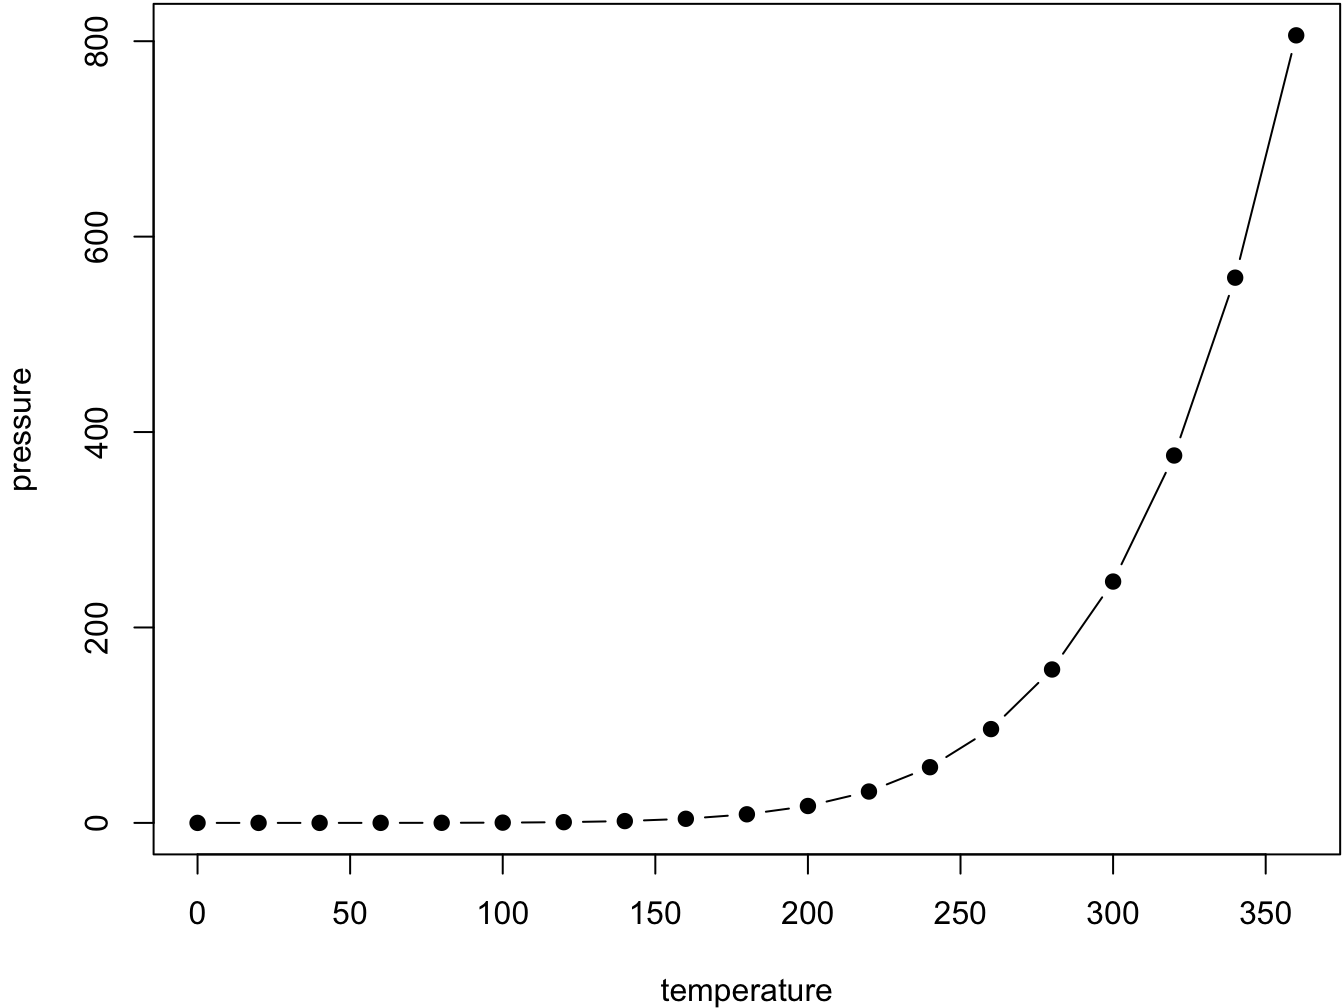
\includegraphics[width=0.8\linewidth]{02-cross-refs_files/figure-latex/nice-fig-1} 

}

\caption{Here is a nice figure!}\label{fig:nice-fig}
\end{figure}

Don't miss Table \ref{tab:nice-tab}.

\begin{Shaded}
\begin{Highlighting}[]
\NormalTok{knitr}\SpecialCharTok{::}\FunctionTok{kable}\NormalTok{(}
  \FunctionTok{head}\NormalTok{(pressure, }\DecValTok{10}\NormalTok{), }\AttributeTok{caption =} \StringTok{\textquotesingle{}Here is a nice table!\textquotesingle{}}\NormalTok{,}
  \AttributeTok{booktabs =} \ConstantTok{TRUE}
\NormalTok{)}
\end{Highlighting}
\end{Shaded}

\begin{table}

\caption{\label{tab:nice-tab}Here is a nice table!}
\centering
\begin{tabular}[t]{rr}
\toprule
temperature & pressure\\
\midrule
0 & 0.0002\\
20 & 0.0012\\
40 & 0.0060\\
60 & 0.0300\\
80 & 0.0900\\
\addlinespace
100 & 0.2700\\
120 & 0.7500\\
140 & 1.8500\\
160 & 4.2000\\
180 & 8.8000\\
\bottomrule
\end{tabular}
\end{table}

\hypertarget{parts}{%
\chapter{Parts}\label{parts}}

You can add parts to organize one or more book chapters together. Parts can be inserted at the top of an .Rmd file, before the first-level chapter heading in that same file.

Add a numbered part: \texttt{\#\ (PART)\ Act\ one\ \{-\}} (followed by \texttt{\#\ A\ chapter})

Add an unnumbered part: \texttt{\#\ (PART\textbackslash{}*)\ Act\ one\ \{-\}} (followed by \texttt{\#\ A\ chapter})

Add an appendix as a special kind of un-numbered part: \texttt{\#\ (APPENDIX)\ Other\ stuff\ \{-\}} (followed by \texttt{\#\ A\ chapter}). Chapters in an appendix are prepended with letters instead of numbers.

\hypertarget{footnotes-and-citations}{%
\chapter{Footnotes and citations}\label{footnotes-and-citations}}

\hypertarget{footnotes}{%
\section{Footnotes}\label{footnotes}}

Footnotes are put inside the square brackets after a caret \texttt{\^{}{[}{]}}. Like this one \footnote{This is a footnote.}.

\hypertarget{citations}{%
\section{Citations}\label{citations}}

Reference items in your bibliography file(s) using \texttt{@key}.

For example, we are using the \textbf{bookdown} package \citep{R-bookdown} (check out the last code chunk in index.Rmd to see how this citation key was added) in this sample book, which was built on top of R Markdown and \textbf{knitr} \citep{xie2015} (this citation was added manually in an external file book.bib).
Note that the \texttt{.bib} files need to be listed in the index.Rmd with the YAML \texttt{bibliography} key.

The RStudio Visual Markdown Editor can also make it easier to insert citations: \url{https://rstudio.github.io/visual-markdown-editing/\#/citations}

\hypertarget{blocks}{%
\chapter{Blocks}\label{blocks}}

\hypertarget{equations}{%
\section{Equations}\label{equations}}

Here is an equation.

\begin{equation} 
  f\left(k\right) = \binom{n}{k} p^k\left(1-p\right)^{n-k}
  \label{eq:binom}
\end{equation}

You may refer to using \texttt{\textbackslash{}@ref(eq:binom)}, like see Equation \eqref{eq:binom}.

\hypertarget{theorems-and-proofs}{%
\section{Theorems and proofs}\label{theorems-and-proofs}}

Labeled theorems can be referenced in text using \texttt{\textbackslash{}@ref(thm:tri)}, for example, check out this smart theorem \ref{thm:tri}.

\begin{theorem}
\protect\hypertarget{thm:tri}{}\label{thm:tri}For a right triangle, if \(c\) denotes the \emph{length} of the hypotenuse
and \(a\) and \(b\) denote the lengths of the \textbf{other} two sides, we have
\[a^2 + b^2 = c^2\]
\end{theorem}

Read more here \url{https://bookdown.org/yihui/bookdown/markdown-extensions-by-bookdown.html}.

\hypertarget{callout-blocks}{%
\section{Callout blocks}\label{callout-blocks}}

The R Markdown Cookbook provides more help on how to use custom blocks to design your own callouts: \url{https://bookdown.org/yihui/rmarkdown-cookbook/custom-blocks.html}

\hypertarget{sharing-your-book}{%
\chapter{Sharing your book}\label{sharing-your-book}}

\hypertarget{publishing}{%
\section{Publishing}\label{publishing}}

HTML books can be published online, see: \url{https://bookdown.org/yihui/bookdown/publishing.html}

\hypertarget{pages}{%
\section{404 pages}\label{pages}}

By default, users will be directed to a 404 page if they try to access a webpage that cannot be found. If you'd like to customize your 404 page instead of using the default, you may add either a \texttt{\_404.Rmd} or \texttt{\_404.md} file to your project root and use code and/or Markdown syntax.

\hypertarget{metadata-for-sharing}{%
\section{Metadata for sharing}\label{metadata-for-sharing}}

Bookdown HTML books will provide HTML metadata for social sharing on platforms like Twitter, Facebook, and LinkedIn, using information you provide in the \texttt{index.Rmd} YAML. To setup, set the \texttt{url} for your book and the path to your \texttt{cover-image} file. Your book's \texttt{title} and \texttt{description} are also used.

This \texttt{gitbook} uses the same social sharing data across all chapters in your book- all links shared will look the same.

Specify your book's source repository on GitHub using the \texttt{edit} key under the configuration options in the \texttt{\_output.yml} file, which allows users to suggest an edit by linking to a chapter's source file.

Read more about the features of this output format here:

\url{https://pkgs.rstudio.com/bookdown/reference/gitbook.html}

Or use:

\begin{Shaded}
\begin{Highlighting}[]
\NormalTok{?bookdown}\SpecialCharTok{::}\NormalTok{gitbook}
\end{Highlighting}
\end{Shaded}


  \bibliography{book.bib,packages.bib}

\end{document}
